%% abtex2-modelo-trabalho-academico.tex, v-1.9.2 laurocesar
%% Copyright 2012-2014 by abnTeX2 group at http://abntex2.googlecode.com/ 
%%
%% This work may be distributed and/or modified under the
%% conditions of the LaTeX Project Public License, either version 1.3
%% of this license or (at your option) any later version.
%% The latest version of this license is in
%%   http://www.latex-project.org/lppl.txt
%% and version 1.3 or later is part of all distributions of LaTeX
%% version 2005/12/01 or later.
%%
%% This work has the LPPL maintenance status `maintained'.
%% 
%% The Current Maintainer of this work is the abnTeX2 team, led
%% by Lauro César Araujo. Further information are available on 
%% http://abntex2.googlecode.com/
%%
%% This work consists of the files abntex2-modelo-trabalho-academico.tex,
%% abntex2-modelo-include-comandos and abntex2-modelo-references.bib
%%

% ------------------------------------------------------------------------
% ------------------------------------------------------------------------
% abnTeX2: Modelo de Trabalho Academico (tese de doutorado, dissertacao de
% mestrado e trabalhos monograficos em geral) em conformidade com 
% ABNT NBR 14724:2011: Informacao e documentacao - Trabalhos academicos -
% Apresentacao
% ------------------------------------------------------------------------
% ------------------------------------------------------------------------

\documentclass[
	% -- opções da classe memoir --
	12pt,				% tamanho da fonte
	%openright,			% capítulos começam em pág ímpar (insere página vazia caso preciso)
	%twoside,			% para impressão em verso e anverso. Oposto a oneside
	oneside,			% para impressão em apenas um lado. Oposto a twoside
	a4paper,			% tamanho do papel. 
	% -- opções da classe abntex2 --
	%chapter=TITLE,		% títulos de capítulos convertidos em letras maiúsculas
	%section=TITLE,		% títulos de seções convertidos em letras maiúsculas
	%subsection=TITLE,	% títulos de subseções convertidos em letras maiúsculas
	%subsubsection=TITLE,% títulos de subsubseções convertidos em letras maiúsculas
	% -- opções do pacote babel --
	english,			% idioma adicional para hifenização
	french,				% idioma adicional para hifenização
	spanish,			% idioma adicional para hifenização
	brazil				% o último idioma é o principal do documento
	]{abntex2}

% ---
% Pacotes básicos 
% ---
\usepackage{lmodern}			% Usa a fonte Latin Modern			
\usepackage[T1]{fontenc}		% Selecao de codigos de fonte.
\usepackage[utf8]{inputenc}		% Codificacao do documento (conversão automática dos acentos)
\usepackage{lastpage}			% Usado pela Ficha catalográfica
\usepackage{indentfirst}		% Indenta o primeiro parágrafo de cada seção.
\usepackage{color}				% Controle das cores
\usepackage{graphicx}			% Inclusão de gráficos
\usepackage{microtype} 			% para melhorias de justificação
% ---
		
% ---
% Pacotes adicionais, usados apenas no âmbito do Modelo Canônico do abnteX2
% ---
\usepackage{lipsum}				% para geração de dummy text
% ---

% ---
% Pacotes de citações
% ---
\usepackage[brazilian,hyperpageref]{backref}	 % Paginas com as citações na bibl
\usepackage[alf]{abntex2cite}	% Citações padrão ABNT

% --- 
% CONFIGURAÇÕES DE PACOTES
% --- 

% ---
% Configurações do pacote backref
% Usado sem a opção hyperpageref de backref
\renewcommand{\backrefpagesname}{Citado na(s) página(s):~}
% Texto padrão antes do número das páginas
\renewcommand{\backref}{}
% Define os textos da citação
\renewcommand*{\backrefalt}[4]{
	\ifcase #1 %
		Nenhuma citação no texto.%
	\or
		Citado na página #2.%
	\else
		Citado #1 vezes nas páginas #2.%
	\fi}%
% ---

% ---
% Informações de dados para CAPA e FOLHA DE ROSTO
% ---
\titulo{Arquitetura xAmpa}
\autor{André Fillipi de Góes Silva\\João Gustavo Rogel de Oliveira}
\local{Santa Rita do Sapucaí}
\data{Novembro de 2019}
\orientador{}
\coorientador{}
\instituicao{INATEL - Instituto Nacional de Telecomunicações}
\tipotrabalho{Relatório (Projeto Final)}
% O preambulo deve conter o tipo do trabalho, o objetivo, 
% o nome da instituição e a área de concentração 
\preambulo{Modelo canônico de relatório acadêmico em conformidade com
as normas ABNT}
% ---


% ---
% Configurações de aparência do PDF final

% alterando o aspecto da cor azul
\definecolor{blue}{RGB}{0,48,84}

% informações do PDF
\makeatletter
\hypersetup{
     	%pagebackref=true,
		pdftitle={\@title}, 
		pdfauthor={\@author},
    	pdfsubject={\imprimirpreambulo},
	    pdfcreator={LaTeX with abnTeX2},
		pdfkeywords={abnt}{latex}{abntex}{abntex2}{trabalho acadêmico}, 
		colorlinks=true,       		% false: boxed links; true: colored links
    	linkcolor=blue,          	% color of internal links
    	citecolor=blue,        		% color of links to bibliography
    	filecolor=magenta,      		% color of file links
		urlcolor=blue,
		bookmarksdepth=4
}
\makeatother
% --- 

% --- 
% Espaçamentos entre linhas e parágrafos 
% --- 

% O tamanho do parágrafo é dado por:
\setlength{\parindent}{1.3cm}

% Controle do espaçamento entre um parágrafo e outro:
\setlength{\parskip}{0.2cm}  % tente também \onelineskip

% ---
% compila o indice
% ---
\makeindex
% ---

% ----
% Início do documento
% ----
\begin{document}

% Retira espaço extra obsoleto entre as frases.
\frenchspacing 

% ----------------------------------------------------------
% ELEMENTOS PRÉ-TEXTUAIS
% ----------------------------------------------------------
% \pretextual

% ---
% Capa
% ---
\imprimircapa
% ---

% ---
% Folha de rosto
% (o * indica que haverá a ficha bibliográfica)
% ---
% \imprimirfolhaderosto*
% ---

%FERRIGNO, C. R. A. \textbf{Tratamento de neoplasias ósseas %apendiculares com
%reimplantação de enxerto ósseo autólogo autoclavado associado ao %plasma
%rico em plaquetas}: estudo crítico na cirurgia de preservação de %membro em
%cães. 2011. 128 f. Tese (Livre-Docência) - Faculdade de Medicina %Veterinária e
%Zootecnia, Universidade de São Paulo, São Paulo, 2011.

%\begin{table}[htb]
%\center
%\footnotesize
%\begin{tabular}{|p{1.4cm}|p{1cm}|p{3cm}|p{3cm}|}
%  \hline
%   \textbf{Folha} & \textbf{Linha}  & \textbf{Onde se lê}  & %\textbf{Leia-se}  \\
%    \hline
%    1 & 10 & auto-conclavo & autoconclavo\\
%   \hline
%\end{tabular}
%\end{table}

%\end{errata}
% ---

% ---
% inserir o sumario
% ---
\pdfbookmark[0]{\contentsname}{toc}
\tableofcontents*
\cleardoublepage
% ---



% ----------------------------------------------------------
% ELEMENTOS TEXTUAIS
% ----------------------------------------------------------
\textual

% ----------------------------------------------------------
% Introdução (exemplo de capítulo sem numeração, mas presente no Sumário)
% ----------------------------------------------------------
\chapter*[Introdução]{Introdução}
\addcontentsline{toc}{chapter}{Introdução}
% ----------------------------------------------------------

Este documento foi elaborado como parte do projeto final da disciplina Arquiteturas de Computadores, a fim de esclarecer detalhes sobre o funcionamento de uma nova arquitetura computacional proposta e desenvolvida a partir dos conhecimentos adquiridos nas aulas.

O desenvolvimento da arquitetura foi baseado em arquiteturas existentes, como a MIPS, e teve um caráter essencialmente prático. O projeto contou com a programação de uma máquina virtual capaz de ler arquivos no formato definido (no caso deste projeto, arquivos *.xampa) e realizar a execução baseada nas instruções definidas previamente.

O principal objetivo do projeto é mostrar, de forma simplificada, como é o processo de desenvovimento de uma nova arquitetura de computadores, bem como mostrar quais devem ser as características consideradas durante o planejamento e a melhor forma de otimizar a solução. Além disso, pode-se colocar em prática conhecimentos que até então tinham sido estudados apenas de forma teórica.


% ---
% Descrição Geral
% ---
\chapter{Descrição Geral}
% ---
A arquitetura xAmpa (Arquitetura mãozinha pra cima) é uma arquitetura computacional de 12 bits, composta inicialmente por 8 registradores e 7 instruções. Seu uso principal é voltado para operações simples entre registradores ou entre um registrador e uma constante (valor imediato ou endereço), como operações de soma, multiplicação, carregamento de valores em um registrador e leitura da memória de dados. A máquina virtual responsável pela execução dos comandos foi desenvolvida na linguagem de programação Python.

% ---
% Explicação breve sobre os registradores
% ---
\section{Registradores}

A arquitetura possui 8 registradores, sendo 2 deles de uso específico e os outros 6 de uso geral. A tabela a seguir apresenta os registradores e seu tipo:\\

\begin{table}[htb]
\center
\footnotesize
\begin{tabular}{|p{3cm}|p{3cm}|p{3cm}|}
  \hline
   \textbf{Registrador} & \textbf{Tipo}  & \textbf{Descrição} \\
    \hline
    a0 & Específico & Program Counter\\
    \hline
    a1 & Específico & Zero imediato\\
    \hline
    a2 & Geral & Dados gerais\\
    \hline
    a3 & Geral & Dados gerais\\
    \hline
    a4 & Geral & Dados gerais\\
    \hline
    a5 & Geral & Dados gerais\\
    \hline
    a6 & Geral & Dados gerais\\
    \hline
    a7 & Geral & Dados gerais\\
    \hline
\end{tabular}
\caption{Registradores disponíveis}
\label{table1:sample}
\end{table}

% ---
% Explicação breve sobre as instruções
% ---
\section{Instruções}

A arquitetura possui, a princípio, apenas 7 instruções. As instruções do tipo R permitem operações entre dois registradores, enquanto as instruções do tipo I permitem operações entre um registrador e uma constante. A tabela a seguir mostra o nome das instruções, seu tipo e uma breve descrição de seu funcionamento:\\ \\ \\ \\ \\ \\

\begin{table}[htb]
\center
\footnotesize
\begin{tabular}{|p{2cm}|p{2cm}|p{10cm}|}
  \hline
   \textbf{Nome} & \textbf{Tipo}  & \textbf{Descrição} \\
    \hline
    SPC & I & Armazena uma constante em um registrador.\\
    \hline
    TCHAN & R & Move o valor de um registrador para outro.\\
    \hline
    ARAKETU & R & Realiza o "ou-exclusivo" entre dois registradores.\\
    \hline
    PSIRICO & R & Realiza a soma entre dois registradores.\\
    \hline
    EVA & I & Realiza a multiplicação entre um registrador e uma constante.\\
    \hline
    ASA & I & Salva um registrador na memória de dados.\\
    \hline
    IVETE & I & Carrega um valor da memória de dados.\\
    \hline
\end{tabular}
\caption{Instruções disponíveis}
\label{table2:sample}
\end{table}

% ---
% Explicação breve sobre a memória cache
% ---
\section{Memória Cache}

A memória cache utilizada na arquitetura é uma memória de instruções, que permite uma velocidade maior na consulta das instruções por dispensar a memória principal caso a instrução desejada esteja salva na memória cache. A cache guarda o endereço da instrução em 4 blocos. Além disso, cada bloco é composto de dois campos: um deles armazena a instrução, enquanto o outro registra a tag da instrução (seu endereço na memória principal).

O ciclo de busca da instrução funciona da seguinte forma: após a identificação da instrução, a máquina virtual acessa a memória cache e checa se a instrução se encontra lá. Em caso afirmativo, a instrução é executada, e em caso negativo, a memória principal é consultada e um bloco com 4 instruções (incluindo a instrução desejada) é carregado na memória cache.

% ---
% Principais componentes
% ---
\chapter{Principais Componentes}
% ---

% ---
% Registradores
% ---
\section{Registradores}

A arquitetura xAmpa possui 8 registradores, sendo 2 deles de uso específico e os outros 6 de uso geral. Os dois registradores de uso específico disponíveis são o a0 e o a1, sendo o primeiro responsável por registrar o Program Counter
e o segundo por possuir o zero imediato. Os outros registradores são de uso geral, para quaisquer dados que sejam armazenados. 

A estrutura dos registradores consiste em um dicionário, cujas chaves são os nomes dos registradores e os valores são variáveis inteiras que armazenam os valores da forma decimal. Além disso, um dicionário auxiliar possui as informações de conversão do nome do registrador para seu identificador no sistema binário.

A tabela a seguir apresenta os identificadores de cada registrador, junto com os dados apresentados anteriormente:\\

\begin{table}[htb]
\center
\footnotesize
\begin{tabular}{|p{3cm}|p{3cm}|p{3cm}|p{3cm}|}
  \hline
   \textbf{Registrador} & \textbf{Tipo} & \textbf{Identificador} & \textbf{Descrição} \\
    \hline
    a0 & Específico & 000 & Program Counter\\
    \hline
    a1 & Específico & 001 & Zero imediato\\
    \hline
    a2 & Geral & 010 & Dados gerais\\
    \hline
    a3 & Geral & 011 & Dados gerais\\
    \hline
    a4 & Geral & 100 & Dados gerais\\
    \hline
    a5 & Geral & 101 & Dados gerais\\
    \hline
    a6 & Geral & 110 & Dados gerais\\
    \hline
    a7 & Geral & 111 & Dados gerais\\
    \hline
\end{tabular}
\caption{Detalhes dos registradores}
\label{table3:sample}
\end{table}

% ---
% Instruções
% ---
\section{Instruções}

A arquitetura possui 7 instruções, responsáveis por operações de registro, carregamento, modificação, soma e multiplicação. As instruções do tipo R permitem operações entre dois registradores, enquanto as instruções do tipo I permitem operações entre um registrador e uma constante. 

A tabela a seguir mostra a estrutura das instruções do tipo I e como deve ser feita a conversão entre a linha de comando em xAmpa e a palavra binária que define a instrução:\\

\begin{table}[htb]
\center
\footnotesize
\begin{tabular}{|p{2.5cm}|p{4cm}|p{5cm}|}
  \hline
   \textbf{op-code} & \textbf{Rd} & \textbf{Imm/Adress}\\
    \hline
    op-code - 3 bits & Registrador destino - 3 bits & Constante ou Endereço - 6 bits\\
    \hline
\end{tabular}
\caption{Instruções do tipo I}
\label{table4:sample}
\end{table}

A próxima tabela mostra a estrutura das instruções do tipo R e como deve ser feita a conversão entre a linha de comando em xAmpa e a palavra binária que define a instrução:\\

\begin{table}[htb]
\center
\footnotesize
\begin{tabular}{|p{2.5cm}|p{4cm}|p{3.5cm}|p{3.5cm}|}
  \hline
   \textbf{op-code} & \textbf{Rd} & \textbf{Rs} & \textbf{Rt}\\
    \hline
    op-code - 3 bits & Registrador destino - 3 bits & Registrador 1 - 3 bits & Registrador 2 - 3 bits\\
    \hline
\end{tabular}
\caption{Instruções do tipo R}
\label{table5:sample}
\end{table}

Na máquina virtual, as instruções estão salvas em um dicionário, cujas chaves são o nome da própria instrução, e o valor é uma lista que possui como primeiro elemento o op-code da instrução e como segundo elemento o tipo da instrução. A tabela a seguir apresenta os op-codes de cada instrução, junto com as informações apresentadas anteriormente:\\

\begin{table}[htb]
\center
\footnotesize
\begin{tabular}{|p{2cm}|p{2cm}|p{1cm}|p{9.5cm}|}
  \hline
   \textbf{Nome} & \textbf{OP-CODE} & \textbf{Tipo} & \textbf{Descrição} \\
    \hline
    SPC & 000 & I & Armazena uma constante em um registrador.\\
    \hline
    TCHAN & 001 & R & Move o valor de um registrador para outro.\\
    \hline
    ARAKETU & 010 & R & Realiza o "ou-exclusivo" entre dois registradores.\\
    \hline
    PSIRICO & 011 & R & Realiza a soma entre dois registradores.\\
    \hline
    EVA & 100 & I & Realiza a multiplicação entre um registrador e uma constante.\\
    \hline
    ASA & 101 & I & Salva um registrador na memória de dados.\\
    \hline
    IVETE & 110 & I & Carrega um valor da memória de dados.\\
    \hline
\end{tabular}
\caption{Detalhes das instruções}
\label{table6:sample}
\end{table}

% ---
% Memória cache
% ---
\section{Memória Cache}

A máquina virtual possui uma memória cache de instruções, responsável por facilitar o ciclo de busca durante a execução do código e melhorar o desempenho. A cache guarda as instruções em blocos, na máquina virtual foi implementada uma cache com 4 blocos. Além disso, para cada bloco existem mais dois campos: um deles armazena a instrução, enquanto o outro registra a tag da instrução (seu endereço na memória principal).

O mapeamento utilizado na implementação da cache é o totalmente associativo, sendo assim cada bloco possui um lugar específico.

A implementação da memória cache foi baseada em duas classes, uma delas responsável por definir o armazenamento e outra responsável pelos blocos de controle. A classe Cache também é responsável pelas funções de busca e carregamento das informações.

% ---
% Funcionamento
% ---
\chapter{Funcionamento}
% ---

% ---
% Ferramentas
% ---
\section{Ferramentas}

O desenvolvimento do projeto contou com o uso da linguagem de programação Python em conjunto com a IDE Microsoft Visual Studio Code.

% ---
% Explicação breve sobre as instruções
% ---
\section{Execução da Máquina Virtual}

O código da máquina virtual é dividido em várias funções, cada uma responsável por uma das etapas da execução. No início do processo, é solicitado ao usuário o caminho do arquivo e se existe a necessidade de mostrar o debug. Após isso, a memória de dados é iniciada e o ciclo de busca se inicia.

No ciclo de busca, o programa é lido e os comandos são separados de acordo com o espaçamento do programa. Em seguida, as palavras binárias para a execução são montadas através de consultas aos registradores, que indicam qual é o código binário correspondente a cada um, bem como o op-code de cada comando, e a memória de programa é atualizada antes do retorno à função principal.

Após a busca, o ciclo de execução é iniciado, a memória cache é configurada e o Program Counter é inicializado com o primeiro endereço para execução. Enquanto houverem dados na memória de programa, o Program Counter é atualizado e a instrução é executada. A palavra binária é dividida em partes menores, correspondentes a cada informação presente na linha de código, e uma série de comandos if-else é responsável por identificar qual é a operação que deve ser realizada. Essa busca da instrução é feita primeiramente na memória cache. Se a instrução desejada estiver carregada (cache hit), ela é executada a partir dali, mas em caso negativo (cache miss), a instrução é buscada na memória principal e carregada na memória cache. Quando ela é identificada, o código identifica os registradores e/ou constantes que serão utilizados e lê os valores que estão salvos. Por fim, a máquina virtual realiza de fato a operação, alterando os registradores necessários. 

Caso o usuário opte por exibir as ferramentas de debug, elas serão mostradas ao final da execução de cada linha, mostrando o estado atual de todos os registradores. Ao final da execução do programa, os registradores são apresentados novamente, indicando qual foi o estado final do processo.

% Ferramentas
% ---
\section{Fluxograma}

O fluxograma a seguir mostra a execução da máquina virtual, a fim de tornar mais simples a visualização do processo:\\

\begin{figure}[h]
\begin{center}
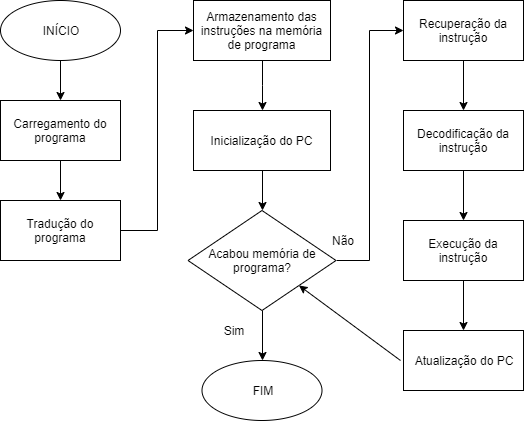
\includegraphics[width=0.8\textwidth]{FluxAmpa}
\end{center}
\caption{Fluxograma do ciclo de execução}
\end{figure}

% ----------------------------------------------------------
% Finaliza a parte no bookmark do PDF
% para que se inicie o bookmark na raiz
% e adiciona espaço de parte no Sumário
% ----------------------------------------------------------
%\phantompart

% ---
% Conclusão (outro exemplo de capítulo sem numeração e presente no sumário)
% ---
\chapter*[Conclusão]{Conclusão}
\addcontentsline{toc}{chapter}{Conclusão}
% ---

Durante a execução do projeto final da disciplina de Arquiteturas de Computadores, foi possível ter uma visão nova de como uma linguagem de programação é executada atráves do desenvolvimento de uma máquina virtual capaz de interpretar um código, e não apenas escrever esse código com uma linguagem de baixo nível. Desta forma, o conhecimento teórico foi posto em prática, e foi possível compreender de forma satisfatória como fatores relacionados ao tamanho da palavra da arquitetura ou a forma como as instruções são implementadas alteram a complexidade da implementação dessa arquitetura.

A implementação foi realizada com sucesso para as primeiras instruções, e existe uma possibilidade de expansão dos comandos caso seja necessário ou desejado no futuro. Além disso, as instruções disponíveis já permitem que programas simples possam ser executados corretamente, mostrando que o projeto pode sim ser utilizado no mundo real, com as adaptações necessárias.

Por fim, é possível dizer que a experiência adquirida com este projeto é de grande importância para a vida acadêmica e profissional dos alunos, por trazer um problema do mundo real e propor uma solução eficaz e capaz de resolvê-lo.


% ----------------------------------------------------------
% ELEMENTOS PÓS-TEXTUAIS
% ----------------------------------------------------------
\postextual
% ----------------------------------------------------------

% ----------------------------------------------------------
% Referências bibliográficas
% ----------------------------------------------------------
\bibliography{abntex2-modelo-references}

% ----------------------------------------------------------
% Anexos
% ----------------------------------------------------------

% ---
% Inicia os anexos
% ---
\begin{anexosenv}

% Imprime uma página indicando o início dos anexos
%\partanexos

% ---
\chapter{Código Fonte da Máquina Virtual}
% ---
O código fonte com a máquina virtual se encontra no GitHub, que pode ser acessado com o link \url{https://github.com/Orange-Caramel/xAmpa}.



%REPOSITÓRIO xAmpa - GitHub. [S. l.], 2019. Disponível em: https://github.com/Orange-Caramel/xAmpa. Acesso em: 26 nov. %2019.


\end{anexosenv}

%---------------------------------------------------------------------
% INDICE REMISSIVO
%---------------------------------------------------------------------
%\phantompart
\printindex
%---------------------------------------------------------------------

\end{document}
